\chapter{Background}
\label{cha:background}

% Software vs. Security
% Risk and vulnerability and CVEs
% Industrial Control Systems (ICS) and Operational Technology (OT)
% Industrial Internet of Things (IIoT)
% Difference Between IT and OT Security
% Devices and Constraints
% What Is a Security Scan

This chapter contains an explanation of many fundamental terms used in the thesis, without which it would not be possible to fully understand all the covered topics.

\section{Software vs. Security}

A software is a set of programs and data which provides functionalities. Security is understanding and identifying software-induced security risks and how to manage them. Software and functionalities come with certain risks and software security is about managing these.

Therefore, software plays a crucial role in providing security, but it is also one of the relevant sources of security issues and problems. Many times the developers have limited training on this concept or the goal is the speed of the development rather than the attention to the hidden details; as result, security is often considered a secondary factor, because it is a complex and expansive task, hard to evaluate when nothing bad happens but usually too late to evaluate when something bad happens~\cite{marchetto-st-slides}.

A software system is secure if it satisfies specified security objectives, starting from the CIA triad which stands for:
\begin{itemize}
  \item \textbf{Confidentiality}: unauthorized actors cannot have access or read the information;
  \item \textbf{Integrity}: unauthorized actors cannot change or alter the information;
  \item \textbf{Availability}: authorized actors can always have access to the information;
\end{itemize}
The CIA triad is a common model that stands as the basis for the development of security systems. Ideally, when all three objectives have been met, the security profile of the organization is stronger and better equipped to handle threat incidents~\cite{cia-triad}.

Secure software is not only composed of the CIA triad; there are also other objectives like~\cite{marchetto-st-slides}
\begin{itemize}
  \item \textbf{Authentication}: who is performing a task;
  \item \textbf{Authorization}: what is that actor allowed to do;
  \item \textbf{Privacy}: controlling personal information from being shared;
  \item \textbf{Anonymity}: remaining unidentified to others;
  \item \textbf{Non-repudiation}: actor cannot deny having taken an action;
  \item \textbf{Reliability}: the extent to which a software yields consistent and expected results;
  \item \textbf{Audit}: having traces of performed actions in separate systems or places;
  \item \textbf{Monitoring}: observing the system for any unusual activity;
  \item \textbf{Intrusion detection}: detecting unauthorized access;
  \item \textbf{Intrusion prevention}: preventing unauthorized access;
\end{itemize}

Total security is unachievable, but the goal is to minimize the risks and the vulnerabilities. Security is a process, not a product, and it is a continuous process~\cite{marchetto-st-slides}.

\section{Risk vs. vulnerability vs. CVE}

We talked about risks in the previous section, but what is a risk? A risk is the potential that a dangerous situation becomes reality. It is the probability of a threat exploiting a vulnerability and the impact of that event. A risk is a combination of a threat, a vulnerability and an impact.

Safety is about protecting from accidental risks, while security is about mitigating the risk of dangers caused by intentional and malicious actors.

A system is secure as its weakest element. A vulnerability is a weakness in a system that can be exploited by a threat. A threat is a potential danger that can exploit a vulnerability. A threat agent is an actor that can exploit a vulnerability. An attack is the exploitation of a vulnerability by a threat agent. An exploit is the code that takes advantage of a vulnerability. A graphical flow of these concepts is shown in~\cref{fig:security-meta-model-def}.

\begin{figure}[ht]
  \centering
  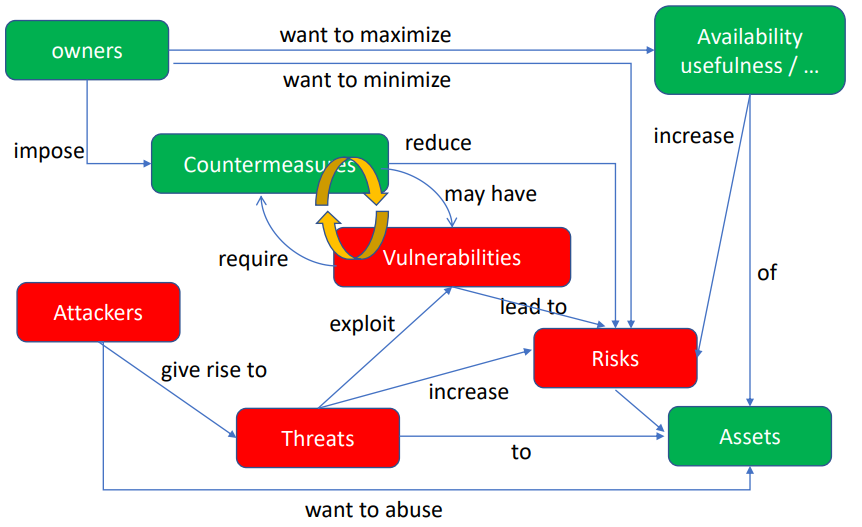
\includegraphics[scale=0.6]{chapters/02/assets/security-meta-model-def}
  \caption[Security meta-model definition]{Security meta-model definition. Image by prof. A. Marchetto taken from \texttt{commoncriteriaportal.org}}
  \label{fig:security-meta-model-def}
\end{figure}

CVE, which stands for \textit{Common Vulnerabilities and Exposures}, is a list of publicly known cybersecurity vulnerabilities. The CVE system provides a reference method for publicly known information-security vulnerabilities and exposures. Each CVE entry represents a unique identifier for a specific vulnerability, named \textit{CVE-ID}, making it easier to reference it across different tools.

Each CVE entry is evaluated using the CVSS score, which stands for \textit{Common Vulnerability Scoring System}. This system provides a standardized way to assess the severity of vulnerabilities. It is important to note that CVSS measures severity, not risk. The difference is that severity is the intrinsic characteristic of a vulnerability while risk is the likelihood of an attacker exploiting the vulnerability and the impact of that event in a specific environment.\\
CVSS v2.0 and CVSS v3.x include three metric groups: Base, Temporal and Environmental. The Base metrics evaluate the intrinsic characteristics of a vulnerability that are constant over time and across user environments. The Temporal metrics adjust the valutation based on factors like patch availability and exploit code and the Environmental metrics allow organizations to customize the score based on their unique environment. The latest version, CVSS v4.0, introduced in 2023, includes Base, Threat, Environmental and Supplemental metric groups. Compared to the previous version, the Threat metrics evaluate the likelihood of an attacker exploiting the vulnerability, the Environmental metrics evaluate the impact of the vulnerability on the organization's unique environment and the Supplemental ones provide additional information about the vulnerability~\cite{cvss-4-spec}.\\
The metrics produce a numerical score from 0 to 10, where highest score means highest severity, and the assessment is also represented as a vector string, which is a concise textual representation of the values used to calculate the score~\cite{cvss-metrics}.

% TODO: Add CVEs for year or some statistics in general

NVD is the \textit{National Vulnerability Database}, a U.S. government database that contains information about known vulnerabilities, including their CVE identifiers and CVSS scores. It is maintained by NIST and serves as a comprehensive resource for organizations to evaluate security risks.

NIST (\textit{National Institute of Standards and Technology}) is a U.S. federal agency that develops cybersecurity standards, guidelines and best practices. Even if it is an American agency, its standards are widely used around the world.

\subsection{Bug}

A bug is a flaw in a system that is not behaving as it is designed to do; a vulnerability is a way of abusing the system, in a security-related way, whether that's due to a design fault or an implementation fault, so a bug.

Many security issues are related to vulnerabilities due to bugs, but not all bugs are vulnerabilities. Exploitation is an activity composed of many steps in which an attacker uses a bug to gain its goal.

\section{IT and OT Security}

IT (\textit{Information Technology}) and OT (\textit{Operational Technology}) focus on protecting different types of systems and they have distinct priorities.

IT is primarily concerned with managing electronic data, supporting business operations and facilitating decision-making through the use of computers and software to securely gather, store, process and share information; basically, it represents the internet access to the cloud we are used to interacting with every day. In contrast, OT focuses on controlling physical processes and equipment in industrial operations such as manufacturing and energy. Unlike IT, OT directly interfaces with industrial machinery and processes, addressing the physical environment and operational requirements~\cite{it-ot-diff-paloalto}, as visible in~\cref{fig:it-ot-diff}.

\begin{figure}[ht]
  \centering
  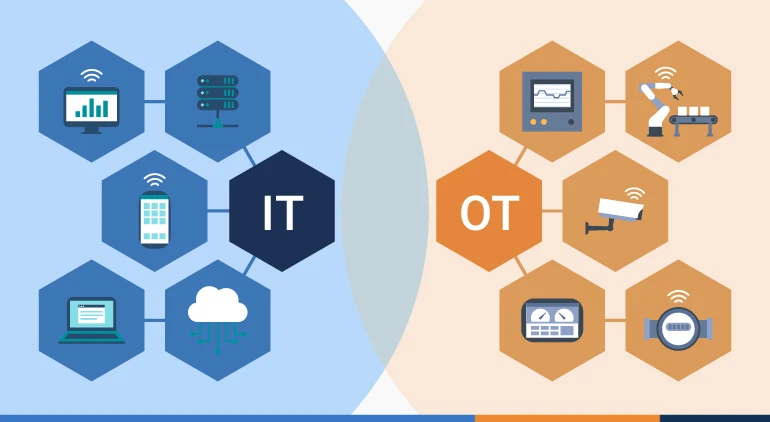
\includegraphics[width=0.9\textwidth]{chapters/02/assets/it-ot-diff}
  \caption[IT vs OT: how they differ]{IT vs OT: how they differ. Image by \texttt{onlogic.com}}
  \label{fig:it-ot-diff}
\end{figure}

We can devise some comparison points between the two types:
\begin{enumerate}
  \item \textbf{Primary priorities}: IT security prioritizes Confidentiality, Integrity and Availability (CIA), with the main focus set to protect data from breaches and authorized actions, while OT security prioritizes Availability, Integrity and Confidentiality (AIC), ensuring the continuous operation of critical systems with safety and reliability being more important than data confidentiality.
  \item \textbf{Impact of Security Breaches}: IT breaches typically affect data confidentiality and may result in privacy violations, financial losses or business disruptions. OT breaches can have severe direct consequences, including physical damage and environmental harm.
  \item \textbf{Security Measures}: IT security can use cybersecurity tools such as firewalls, antivirus, encryption and user authentication. Instead, OT security should require specialized tools like network segmentation, strict access control and real-time monitoring.
  \item \textbf{Regulatory Requirements}: IT uses regulations like GDPR, the \textit{General Data Protection Regulation} to protect personal data for a European citizen and standards like ISO-27001, while OT follows regulations and standards like the IEC 62443, which is a series of standards for industrial automation and control systems management and security. More on these regulations in the next chapters.
  \item \textbf{Vulnerability management}: IT systems can usually be patched with a software update in a short time without severe impact on operations, while OT systems may require a longer time to be patched, as they are often critical to the operation of industrial processes or incompatible with the running legacy systems.
\end{enumerate}

Despite their distinct differences, IT vs. OT cybersecurity share similarities and are increasingly overlapping and one approach has not to exclude the other.

According to~\cref{fig:fortinet-intrusions-env-impacted} taken by the \textit{2023 State of Operational Technology and Cybersecurity Report} by Fortinet\footnote{\url{https://www.fortinet.com}}, a global leader of cybersecurity solutions and services, nearly one-third of respondents indicated both IT and OT systems were impacted, up from the 21\% in 2022.

\begin{figure}[ht]
  \centering
  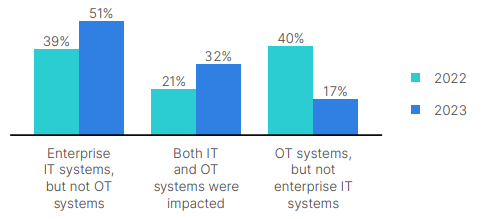
\includegraphics[scale=0.8]{chapters/02/assets/fortinet-intrusions-env-impacted}
  \caption[Attacks to IT and OT systems: impacted environments]{Attacks to IT and OT systems: impacted environments}
  \label{fig:fortinet-intrusions-env-impacted}
\end{figure}


As a general rule, OT devices are traditionally kept separate from the public internet and often internal networks, which means they can only be accessed by authorized employees. However, it is increasingly possible for OT systems to be controlled and monitored by IT systems or remotely via the Internet~\cite{it-ot-cybersecurity}.

\section{Industry 4.0}

Industry 4.0, synonymous of \textit{smart manufacturing}, is the realization of the digital transformation of the field, delivering real-time decision-making, enhanced productivity, flexibility and agility to revolutionize the way companies manufacture, improve and distribute their products.

This is the Fourth Industrial Revolution, characterized by increasing automation and the employment of smart machines and smart factories. By collecting more data from the factory floor and combining that with other enterprise operational data, a smart factory can achieve information transparency and better decisions.

Some specific technologies are pushing this revolution:~\cite{what-is-industry-4-0}
\begin{itemize}
  \item \textbf{Internet of Things (IoT)}: machines on the factory floor are equipped with boards that allow the machines to connect with remote services, making possible for large amounts of valuable data to be collected, analyzed and exchanged.
  \item \textbf{Cloud computing}: the typically large amount of data being stored and analyzed can be processed efficiently and cost-effectively with \textit{the cloud}. Cloud computing can also reduce startup costs for small- and medium-sized manufacturers who can right-size their needs and scale as their business grows.
  \item \textbf{AI and machine learning}: Artificial Intelligence (AI) and machine learning can create insights providing visibility, predictability and automation of operations and business processes. The data collected from these assets can help businesses perform predictive maintenance based on machine learning algorithms, resulting in more uptime and higher efficiency.
  \item \textbf{Edge computing}: to reduce latency and improve security, edge computing can be used to process the needed data closer to the source, rather than sending all the raw statistics to the cloud, wasting bandwidth and time.
  \item \textbf{Cybersecurity}: last but not least, when undergoing a digital transformation to Industry 4.0, it is essential to consider a cybersecurity approach that encompasses IT and OT equipment.
\end{itemize}

\section{Industrial devices: PLC and HMI}

Industrial devices are used in many different sectors like manufacturing, energy, transportation and so on. We can trace back these devices to a common tablet placed on a wall or on a production line, with the difference that these devices support a wide range of industrial protocols. They are usually not connected to the internet and they take input from a physical human interaction physically on the place.

These types of devices are an example of HMI, which stands for \textit{Human Machine Interface}, and they are defined as a feature or component of a certain entity that enables humans to engage and interact with machines. In the past HMIs started to be command line interfaces handled by a keyboard, then they evolved to graphical user interfaces with the support for the mouse navigation and now they are touchscreens, where the end-user directly touches the screen.\\
Traditionally, to integrate a manufacturing line with an HMI, the HMI had to be connected to a \textit{Programming Logic Controller} (PLC) to display the data received from the PLC and give the PLC input from users~\cite{what-is-hmi}.

In terms of the demands of Industry 4.0, industrial HMIs will also see further incorporation of new and emerging technologies that are impacting HMIs as a whole. First of all, there is the need to start integrating the Internet of Things (IoT) into industrial HMIs. This will allow the collection of data from the factory floor and the ability to analyze those data in real-time. This will also allow the ability to control the factory floor from a remote location. Of course, making these devices connected to the internet makes the risks of cyberattacks higher.

\section{ICS and IACS}

ICS and IACS refer respectively to \textit{Industrial Control System} and \textit{Industrial Automation and Control Systems}. In our context, they can be used interchangeably to define the collection of hardware, software and policies that control and manage an industrial process. Basically, it means that anything interacting with the system influencing its safety, security and operations belongs to IACS~\cite{ics-or-iacs}.

We use this terminology in the next chapters, especially related to the security regulations of the systems.

\section{Standards and Regulations}
Until the so-called third industrial age, or Industry 3.0, cybersecurity had minimal impact on manufacturing. Industrial machinery wasn't necessarily connected to the internet or to each other, making external risks unlikely. However, with the dawn of Industry 4.0, smart machinery and smart factories have become vital for the smooth operation of production departments, placing cybersecurity at the forefront of concern.

Cybersecurity involves protecting systems, networks and programs from digital attacks. Given the critical nature of the topic and the attention it demands, companies are embarking on paths to elevate their awareness of cyberattacks, adopting internal policies, or even pursuing specific certifications in cybersecurity. Concurrently, national and international legislators have introduced new legislative measures imposing new obligations on certain entities concerning cybersecurity.

Let's now consider the most recent legislative measures on cybersecurity and the related certifications that manufacturing industries must take into account.\\
Certifications provide a guarantee of product and company security. The main certifications currently considered include:
\begin{itemize}
  \item \textbf{IEC 62443}: This series of international standards is renowned for enhancing the security of industrial control systems, setting forth fundamental prerequisites to shield industrial systems from cyber threats;
  \item \textbf{ISO/IEC 27001 (2022)}: This certification covers various aspects, including security policy, human resource security, physical and environmental security, communications management and regulatory compliance;
\end{itemize}

There are then several laws and regulations that address the issue of cybersecurity under various profiles.

Among them it is worth noting:~\cite{cybersecurity-standards-regulations-compliance}
\begin{itemize}
  \item \textbf{Cyber Resilience Act (CRA)}~\footnote{\url{https://eur-lex.europa.eu/legal-content/EN/TXT/?uri=celex:52022PC0454}}: While still pending final approval by the European Institutions, the Cyber Resilience Act seeks to enhance the resilience of the European digital market by ensuring that connected devices and digital services are equipped to withstand cyberattacks effectively. It will become effective in 2027;
  \item  \textbf{NIS Directive 2}~\footnote{\url{https://eur-lex.europa.eu/legal-content/EN/TXT/?uri=CELEX:32022L2555}}: This directive outlines essential criteria that companies must adhere to in order to maintain a robust level of cybersecurity. These criteria cover the implementation of risk analysis strategies, fortification of information system security and effective incident management protocols. EU Member States must transpose this directive, with enforcement specified in the respective national acts;
  \item \textbf{Italian Cybersecurity Law (June 28th, 2024 No. 90)}~\footnote{\url{https://www.gazzettaufficiale.it/eli/id/2024/07/02/24G00108/sg}}: This Italian law pertains to national cybersecurity and applies to both public and private entities whose services are deemed critical. It mandates the implementation of security measures to protect critical digital infrastructures and sensitive information, including specific obligations to notify the Cybersecurity Agency of any cyber incidents;
  \item \textbf{New Machinery Regulation No. 1230/2023}~\footnote{\url{https://eur-lex.europa.eu/legal-content/EN/TXT/?uri=CELEX:32023R1230}}: This regulation will replace the Machinery Directive No. 2006/42/EC, focusing on the overall safety of machinery and semi-machinery and it will become effective in 2027. It emphasizes the essential integration of cybersecurity into the design and manufacturing processes of machinery, recognizing the potential risks that cyber vulnerabilities pose to physical safety;
\end{itemize}

\section{Security vulnerabilities scan}

A security vulnerabilities scan is a process that looks for vulnerabilities in a system or network. It is a way to identify potential security risks and weaknesses that could be exploited by attackers. The scans can be performed manually or automatically using specialized tools. The goal of this type of scan is to identify vulnerabilities and provide recommendations for improving the security of the system.

There are also different types of security scans, including network scans and penetration tests. Network scans are used to identify devices on a network and detect open ports and services while penetration tests are used to simulate cyberattacks and test the security of a system.

Security scans are an important part of a comprehensive security program. They can help organizations identify and address security vulnerabilities before they are exploited by attackers. By regularly performing security scans, organizations can improve their security attitude and reduce the risk of a security breach.

\section{JSON and YAML}

JSON, acronym of \textit{JavaScript Object Notation}, is a lightweight data-interchange format that is easy for humans to read and write and easy for machines to parse and generate. It is based on a subset of the JavaScript programming language. JSON is often used to exchange data between a server and a web application. It is a text format that is language-independent and can be used with any programming language. JSON is commonly used for configuration files, API responses and data storage.

YAML, a recursive acronym of \textit{YAML Ain't Markup Language}, is a human-readable data serialization format that is usually used for configuration files. It is a superset of JSON and is designed to be more human-readable and easier to write than JSON. It is commonly used in the cloud computing industry for configuration files and infrastructure as code.

\noindent\begin{minipage}{\linewidth}
  \vspace{0.5cm}
  \begin{lstlisting}[style=json, caption={JSON example}, label={lst:json-example}]
{
  "name": "John",
  "employed": true,
  "address": {
    "city": "Verona",
    "country": "Italy"
  },
  "hobby": ["reading", "running"]
}
  \end{lstlisting}
\end{minipage}

\noindent\begin{minipage}{\linewidth}
  \vspace{0.5cm}
  \begin{lstlisting}[style=yaml, caption={YAML example}, label={lst:yaml-example}]
name: John
employed: true
address:
  city: Verona
  country: Italy
hobby:
  - reading
  - running
  \end{lstlisting}
\end{minipage}

The example in~\cref{lst:json-example} shows the data represented in JSON, while~\cref{lst:yaml-example} shows the same data as YAML.

\section{REST API}

REST stands for \textit{REpresentational State Transfer}, and it is an architectural style for designing networked applications. It relies on a stateless client-server communication protocol, meaning that each request from a client to a server must contain all the information necessary to understand that request. REST is usually used in web services development as a way to communicate between client and server.

A REST API is an application programming interface that uses HTTP requests to perform operations on a server. The endpoints can be called in a RESTful way, meaning that the user transfers a representation of the state of the resource to the destination endpoint with appropriate HTTP methods to perform standard functions like creating, reading, updating and deleting records (also known as \textit{CRUD}) within a resource~\cite{rest-api}.

\section{Microservices deployment}

This section explains how software can be deployed in a cloud environment, with a focus on the microservices architecture.

\subsection{Microservice}

Microservice architecture is an architectural style that organizes an application into a set of services that can be deployed independently and are loosely coupled. This means each service is packaged as an executable unit ready for production; in addition, services do not have direct dependencies on each other, allowing for independent development, deployment and scaling on the needs~\cite{microservices-what-are}.

In doing so, there is no need to scale or deploy the entire application when only a part of it needs to be updated or scaled. This approach allows for faster development and deployment cycles, as well as improved fault tolerance and scalability. The concept is shown in~\cref{fig:monolith-microservices}.

\begin{figure}[ht]
  \centering
  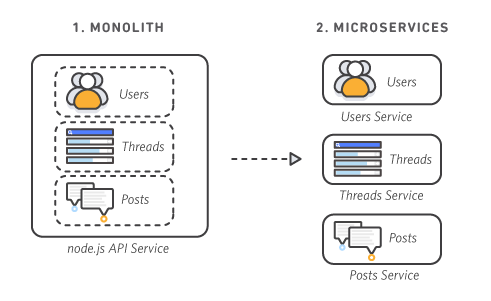
\includegraphics[scale=0.6]{chapters/02/assets/monolith-microservices}
  \caption[Breaking a monolithic application into microservices]{Breaking a monolithic application into microservices. Image by \texttt{aws.amazon.com}}
  \label{fig:monolith-microservices}
\end{figure}

\subsection{Virtualization}

Virtualization is a technology that enables the creation of virtual versions of physical resources such as processors, storage devices, or network components. By simulating the functions of physical hardware, virtualization allows multiple operating systems to run on a single physical machine. This approach enhances IT agility, flexibility and scalability, while also providing significant cost savings by abstracting the underlying physical hardware~\cite{virtualization-aws}.

Each virtualized environment runs within its allocated resources. There are two main types of virtualization approaches: container-based virtualization and hypervisor-based virtualization, also known as virtual machines' virtualization.

\subsubsection{Container vs. Virtual Machine}

A modern and efficient way to execute microservices is to use \textit{containers}. \\
Containers are lightweight software packages that contain all the dependencies required to execute the contained software application in a virtualized environment. They share the same kernel of the host system, but they are usually isolated from the host and from other containers and they can run different operating systems. Another advantage of containers is that they are immutable, meaning that they could be altered after their execution, but the state is restored at each restart.\\
Instead, compared to the containers, \textit{virtual machines}'s goal is to virtualize the entire system hardware, therefore they are slower and heavier - resources side and disk usage side - than containers.

Since we are talking of a microservices architecture, there is the need to run multiple containers at the same time, and to manage them, from the creation to the destruction up to the recovery in case of failure or the scaling in case of high load. This is where we need an orchestration tool.

\subsection{Orchestration}

Orchestration is a term referring to the automated configuration, coordination and management of virtualization software. It is used to manage the deployment, scaling and operation of application containers. Orchestration tools are used to automate the deployment and scaling of containers, as well as to manage the networking, the storage configurations of the containers and much more. The most popular orchestration tool is Kubernetes.

\subsection{CI/CD}

A container is a running instance of an image, that is an executable package that includes all the needed software, libraries and dependencies to run an application. Images are mainly built from a Dockerfile, which is a configuration file that contains a series of instructions describing how the image should be built. Tipical steps are the installation of a base image and the runtime software along with the application code, otherwise another alternative could be to directly embed an executable file. Each specific modification or addition, such as installing a new package, represents a new layer in the image. The layering layout allows for their caching and reuse, making the building process faster and more efficient in case of changes.\\
The building process can be automated by a \textit{Continuous Integration} (CI) tool. Later, the images must be pushed to a registry, that is a repository where the images are stored. The deployment of the images can be automated by a \textit{Continuous Deployment} (CD) tool.

CI and CD are practices that allow the developers to automate the building, testing and deployment of the software. CI is the practice of integrating the code changes of the developers into a shared repository multiple times a day, and CD is the practice of automatically deploying the code changes to the production environment. CI/CD allows the developers to detect and fix the bugs early, to reduce the risk of integration issues and to deliver the software faster and more frequently.

% terraform?

\section{Agile method}

The \textit{Agile methodology} is a project management philosophy that involves breaking the project into phases and emphasizing continuous collaboration and improvement. Teams follow a cycle of planning, executing and evaluating. Teams choose agile so they can respond to changes in the market or feedback from customers quickly without derailing a year's worth of plans. The publication of the Agile Manifesto\footnote{\url{https://agilemanifesto.org}} in 2001 marks the birth of the methodology. Since then, many agile frameworks have emerged such as scrum, kanban or lean. Each embodies the core principles of frequent iteration, continuous learning and high quality in its own way~\cite{agile-methodology}.

\subsection{Scrum}

Scrum is an agile project management framework, which is different from Agile, a philosophy.\\
The definition of scrum is based on empiricism and lean thinking. Empiricism says that knowledge comes from experience and that decisions are made based on what is observed. Lean thinking reduces waste and focuses on essentials. The scrum framework is heuristic; it is based on continuous learning and adjustment to fluctuating factors by acknowledging that the team does not know everything at the start of a project and it will evolve through experience. Scrum is structured to help teams to naturally adapt to changing conditions and user requirements, with re-prioritization built into the process and short release cycles so your team can constantly learn and improve~\cite{scrum}.

Scrum artefacts help to define the product, what work has to be done to create it and who has to do it. An \textit{epic} is a large body of work that can be broken down into smaller tasks. Each of these tasks is called \textit{story} and it is a short requirement written from the perspective of an end user. The story is linked to a person in the team that has to carry it out.

The two main artefacts boards are the \textit{product backlog} and the \textit{sprint backlog}. \\
The former is a list of all the tasks that needs to be done; it is a dynamic list of features, requirements, improvements, fixes and epics, ordered by their priority. Essentially, it is a \textit{"To Do"} list.\\
The latter is a list of items selected for the current sprint cycle; the sprint cycle is a fixed period of time, usually up to four weeks. Before each sprint, the team selects items from the product backlog to work on. Epics are broken down into stories and stories are moved from the product backlog to the sprint backlog~\cite{scrum-epic-stories}.

\begin{figure}[ht]
  \centering
  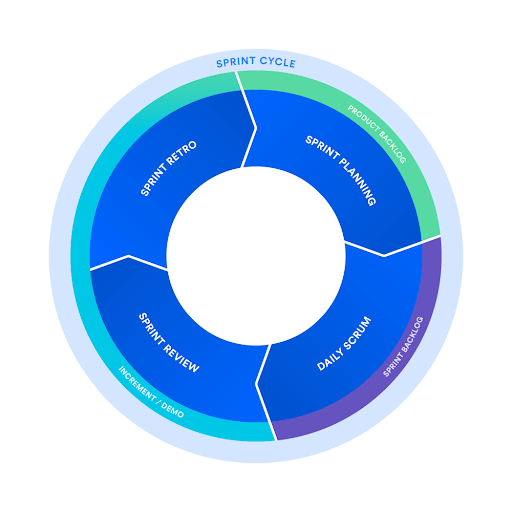
\includegraphics[width=0.8\textwidth]{chapters/02/assets/scrum}
  \caption[Scrum sprint cycle]{Scrum sprint cycle. Taken from \texttt{atlassian.com}}
  \label{fig:scrum-sprint-cycle}
\end{figure}

As visible in~\cref{fig:scrum-sprint-cycle}, Scrum is split in four principal phases:
\begin{itemize}
  \item The \textbf{sprint planning} is the initial phase of a sprint, the actual time period when the scrum team works; the team meets and decides what to do in the sprint by placing the tasks from the product backlog to the sprint backlog;
  \item The \textbf{daily scrum} is a daily meeting where the team members synchronize with each other. It is usually taken stand-up, as a way to not waste time and to keep the meeting short;
  \item The \textbf{sprint review} and \textbf{sprint retrospective} are the meetings at the end of the sprint where the team shows what they have done and demonstrates the work to the stakeholders and receive feedback;
\end{itemize}
